%----------------------------------------------------------------------------
% 4. Rendszerterv ismertetése
%
% A tervezés részletes leírása, a döntési lehetőségek értékelése és a
% választott megoldások indoklása

%\chapter{Introduction}
%\chapter{Earlier monitoring systems implemented in the dormitory}
%\chapter{Requirements of the new monitoring system}
%\chapter{Available industry standard technologies}
\chapter{System architecture \label{ch4}}
%\chapter{Implementation details and experiences}
%\chapter{Results and evaluation}
%\chapter{Future development opportunities}
%----------------------------------------------------------------------------

As discussed in the previous chapter we have decided to use VictoriaMetrics,
Loki, Promtail and Grafana for our new monitoring system. Let's see the new
system architecture.

%----------------------------------------------------------------------------
\section{System Components}
%----------------------------------------------------------------------------

%\begin{lstlisting}
%              VMAlertmanager                                     %
%                    |                                            %
%                 VMAlert                                         %
%                    |                                            %
%                 VMSingle ------- VMAgent ------ { exporters }   %
%                    |                                            %
% { users } ----- Grafana                                         %
%                    |                                            %
%                   Loki --------- Promtail ---- { remote hosts } %
%\end{lstlisting}

\begin{figure}[!h]
	\centering
	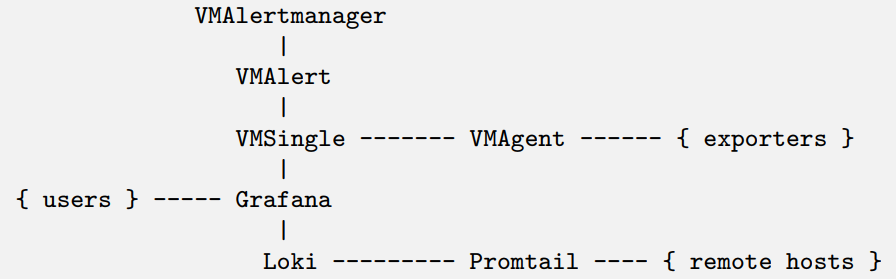
\includegraphics[width=150mm, keepaspectratio]{figures/arch-left.png}
	\caption{System Components}
%	\label{fig:mesh1}
\end{figure}

\subsection{VictoriaMetrics Components}

We are going to use VictoriaMetrics for scraping and storing metrics,
generating alerts and sending out notifications.

As \kszk's infrastructure is small compared to what VictoriaMetrics is able to
handle we have opted for a simple deployment. This type of deployment uses one
service of each type which is easier to configure and handle at the cost of
scalability. We do not expect to hit any bottlenecks with this choice.

\subsubsection{VMAgent}

The VMAgent component pulls metrics from exporters installed on remote hosts.
The list of targets is defined by it's own configuration. Scraped metrics are
then sent to the VMSingle component.

\subsubsection{VMSingle}

The VMSingle component is the central time series database of VictoriaMetrics.
This stores collected metrics and exposes them via an HTTP API. This single
service is basically the cluster version's 3 components (\verb+vminsert+,
\verb+vmstorage+, \verb+vmselect+) compiled into one.

\subsubsection{VMAlert}

The VMAlert component reads metrics from the VMSingle component. Based on it's
configured rules it decides whether the conditions to fire an alert are met. If
an alert fires it is sent to the VMAlertmanager component.

If recording rules are configured it is able to write the results of complex
queries back to VMSingle. This is useful if we want to precalculate time
consuming queries which can later be accessed just like regular metrics.

\subsubsection{VMAlertmanager}

The VMAlertmanager component receives alerts from the VMAlert component. Then
based on it's alert routing and receivers configurations it decides if a
notification should be sent. If conditions are met a notification is sent out
to one or more external services, most importantly to \kszk's Mattermost
(not pictured) server.

\subsection{Promtail}

Promtail receives and processes logs from remote hosts. Unlike VictoriaMetrics
remote hosts push their logs to Promtail. Promtail then sends the processed
logs to Loki.

\subsection{Loki}

Loki indexes and stores logs received from the Promtail component. It receives
requests from Grafana, queries it's internal datastore and responses with the
results. Just like the VictoriaMetrics TSDB Loki can be installed as multiple
instances of different components or as one single component. The former is
useful for higher volumes of logs while the latter is much more simple to set
up and maintain at the cost of scalability. We have opted for the simpler
method as we do not expect to hit any bottlenecks here either.

\subsection{Grafana}

Grafana is only used for visualizations in our architecture. This is our main
user-facing component: users get authenticated and authorized here. After
logging in they are able to create, view and modify dashboards on Grafana.
Grafana queries Loki and/or VMSingle for the data required by the currently
viewed dashboard(s).

%----------------------------------------------------------------------------
\section{Deployment}
%----------------------------------------------------------------------------

All of the above listed components can be installed in a wide variety of ways.
If needed these can be downloaded separately, compiled from source and then run
as classic Unix daemons. Docker images are also available for each of these. On
the other end of the spectrum these components can easily run on Kubernetes as
vast amounts examples, guides and official configurations are available for
this kind of setup.

\subsection{Kubernetes}

Kubernetes\cite{k} is an open-source system for automating the deployment, scaling, and
management of containerized applications. It is a popular platform for running
microservices and other distributed applications, and is often used in
cloud-native environments. Kubernetes provides a number of features to help you
manage your applications, including automatic scheduling and scaling of
containers, self-healing, and service discovery.

We have decied to opt for Kubernetes because:
\begin{itemize}
	\item freely available documentations and configurations make it very easy to use
	\item Kubernetes handles the lifecycle of jobs and pods for us
	\item as \kszk's members already operate a k8s cluster they have experience using this system
	\item by using Kubernetes we can easily expand the system with new physical servers in the future
\end{itemize}

All in all by installing our software stack on Kubernetes we are able to
implement this architecture much quicker, easier and without the need for
custom tools.
